%!TEX root = Main.tex
\documentclass[Main]{subfiles}

\begin{document}

\section{Contribution} % (fold)
\label{sec:contribution}

	The contribution from this mini-project consists of an implementation and test of the DFTSP.
	\subsection{Implementation} % (fold)
	\label{sub:implementation}

		\subsubsection{DFTSP Mote} % (fold)
		\label{sub:dftsp_mote}
			The DFTSP has been implemented on Crossbow Telosb motes\cite{TelosBDatasheet:Online} running the TinyOS\cite{TinyOS:Online} operating system. 
			The DFTSP implementation builds upon the FTSP implementation already available for TinyOS\cite{FTSPImplementationTinyOS:Online}.
			In Figure \ref{fig:nesdoc_dstfp_app_c} a Nesdoc\cite{Nesdoc:Online} overview of the DFTSP application is shown. 
			The application consists of two major components, which each will be described in the following subsections.
			
			\begin{itemize}
			 	\item TimeSyncC - Handles the DFTSP
			 	\item TestResponderC - Handles all test communication
			\end{itemize}

			\begin{figure}[H]
				\centering
				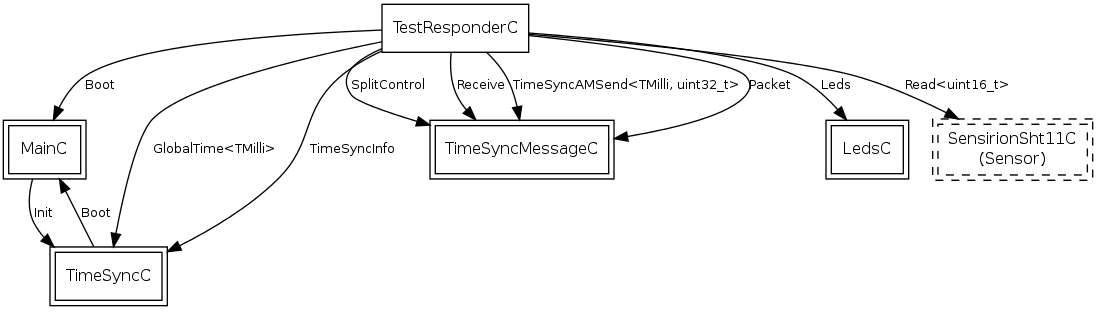
\includegraphics[width=\linewidth]{NesdocDFTSPAppC}
				\caption{DFTSP Application module overview}
				\label{fig:nesdoc_dstfp_app_c}
			\end{figure}

			\paragraph{TimeSyncC} % (fold)
			\label{par:timesyncc}
				The TimeSyncC component was original part of the FTSP implementation, but has been modified and extended to handle the DFTSP.
				In Figure \ref{fig:nesdoc_time_sync_c} an overview of the TimeSyncC component is shown.
				This overview is identical to the FTSP implementation, but the interfaces TimeSyncInfo and TimeSyncMode and the TimeSyncP module have been changed.

				\begin{figure}[H]
					\centering
					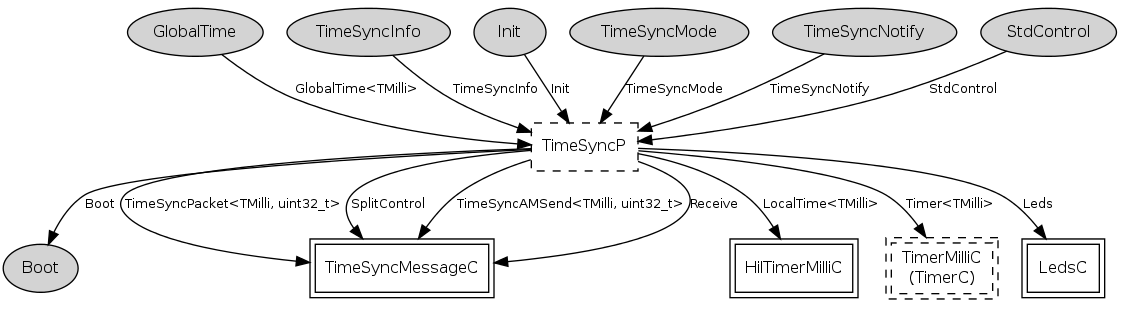
\includegraphics[width=\linewidth]{NesdocTimeSyncC}
					\caption{TimeSyncC module overview}
					\label{fig:nesdoc_time_sync_c}
				\end{figure}

				In DFTSP the parent node must receive broadcast from their children in order to calculate their drift and update its time synchronization period.
				This have numerous impacts on the protocol.
				First of all, the motes needs to include both skew estimation and hop number in the broadcasted time synchronizing messages. 
				The hop number is needed, so that the motes can differentiate between parents, children and neighbors. 
				The skew estimate is needed so that the parent can calculate the drift of its children.
				Secondly, the parent must keep reference about is children and their previous skew estimates, in order to calculate their drift


				TODO
			ChildTable\[MAX\_CHILDREN\]
			-nodeId
			-oldSkew
			-oldTime
			-drift

			childEntries
			beaconPeriod

			UpdateBeaconPeriod()
			handleNewChildSkew()

			hop \& sequence number changes

			Added hop and skew in msg
			\begin{figure}[H]
				\begin{lstlisting}[caption=TimeSyncMsg, style=Code-C, label=lst:time_sync_msg]
			typedef nx_struct TimeSyncMsg
			{
				nx_uint16_t	rootID;		// The node id of the synchronization root
				nx_uint16_t	nodeID;		// The node id of the sender
				nx_uint8_t	seqNum;		// Sequence number for the root
				nx_uint32_t skew;			// Skew 
				nx_uint8_t  hop;			// Hop count from root
				nx_uint32_t	globalTime;
				nx_uint32_t localTime;
			} TimeSyncMsg;
				\end{lstlisting}
			\end{figure}

			New timer mode?


			TimeSyncInfo, Add drift and syncPeriod - only for testing purposes.


			% paragraph timesyncc (end)

			

			
			
			\paragraph{Test Responder Module} % (fold)
			\label{par:test_responder_module}
				The test responder module has been added to the DFTSP application to enable it to participate in the tests.
				An overview given in Figure \ref{fig:DFTSPResponderOverview} shows the modules used.

				\begin{figure}[H]
					\centering
					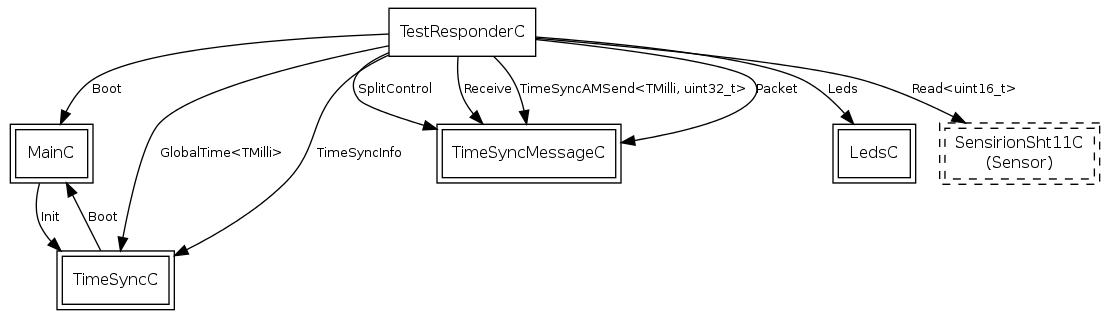
\includegraphics[width=\linewidth]{DFTSPResponderOverview.png}
					\caption{DFTSP Responder Module Overview}
					\label{fig:DFTSPResponderOverview}
				\end{figure}

				The responsibility of the test responder module is to receive the query message from the broadcaster, acquire the necessary data and respond to the broadcaster.
				The data is shown in listing \ref{code:test_data}.

				\begin{figure}[H]
					\begin{lstlisting}[caption=DFTSP Test Data, style=Code-C, label=code:test_data]
		typedef nx_struct SyncReportMsg
		{
			nx_uint16_t	nodeID;			// the node if of the sender
			nx_uint32_t	globalTimeEst;	// the senders estimation of the global time
			nx_uint8_t  syncPeriod;		// the senders synchronization period
			nx_uint32_t  drift;			// the senders estimation of its child's drift
			nx_uint16_t  temp;			// the senders temperature measurement
			nx_uint8_t	seqNum;		// sequence number for the root
		} SyncReportMsg;

					\end{lstlisting}
				\end{figure}

				All fields except the $temp$, which holds the temperature of the mote, are provided by the DFTSP module.
				The temperature is read using the Sensirion SHT11\cite{tempSensorDatasheet} temperature and humidity sensor on the Telosb.
				The module connection, read invoke and readDone event are shown in listing \ref{code:temp_impl}.

				\begin{figure}[H]
					\begin{lstlisting}[caption=Temperature reading implementation, style=Code-C, label=code:temp_impl]
		typedef nx_struct SyncReportMsg
		{
		// Temperature Module Connection
		components new SensirionSht11C() as Sensor;
		App.Read -> Sensor.Temperature;

		// Read invoke
		event message_t* Receive.receive(message_t* msgPtr, void* payload, uint8_t len)
		{
	    	call Read.read();
	    	// Rest of the receive implementation


		// ReadDone event
		event void Read.readDone(error_t result, uint16_t val)
		{
			if(result == SUCCESS)
			temp = val;
		}

						\end{lstlisting}
				\end{figure}
			% paragraph test_responder_module (end)
		% subsubsection dftsp_mote (end)
		
		
		\subsubsection{Broadcaster Mote} % (fold)
		\label{sub:broadcaster_mote}
			The broadcaster application has also been implemented on a Crossbow Telosb mote. 
			An overview of the application given in Figure \ref{fig:broadCastAppOverview} shows the modules used. 

			\begin{figure}[H]
				\centering
				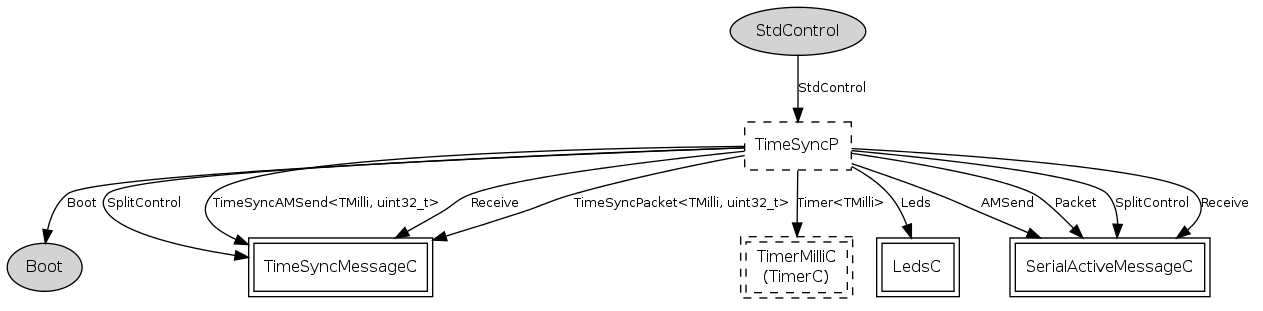
\includegraphics[width=\linewidth]{BroadcastAppOverview.png}
				\caption{Broadcast application overview}
				\label{fig:broadCastAppOverview}
			\end{figure}

			The broadcaster application is also based on the FTSP implementation given in \cite{FTSPImplementationTinyOS:Online}.	
			Periodically, at the $BROADCAST\_RATE$, the broadcaster mote will query the DFTSP parent and child for the data shown in listing \ref{code:test_data}.
			Upon reception, the broadcaster application sends the data to the test PC using a USB connection, as seen in Figure \ref{fig:TestSetup}.

		% subsubsection broadcaster_mote (end)
	

		
		\subsubsection{Serial Java Application} % (fold)
		\label{sub:serial_java_application}
		
		% subsection serial_java_application (end)

	% subsection implementation (end)

	\subsection{Test Setup} % (fold)
	\label{sub:test_setup}

		\begin{figure}[H]
			\centering
			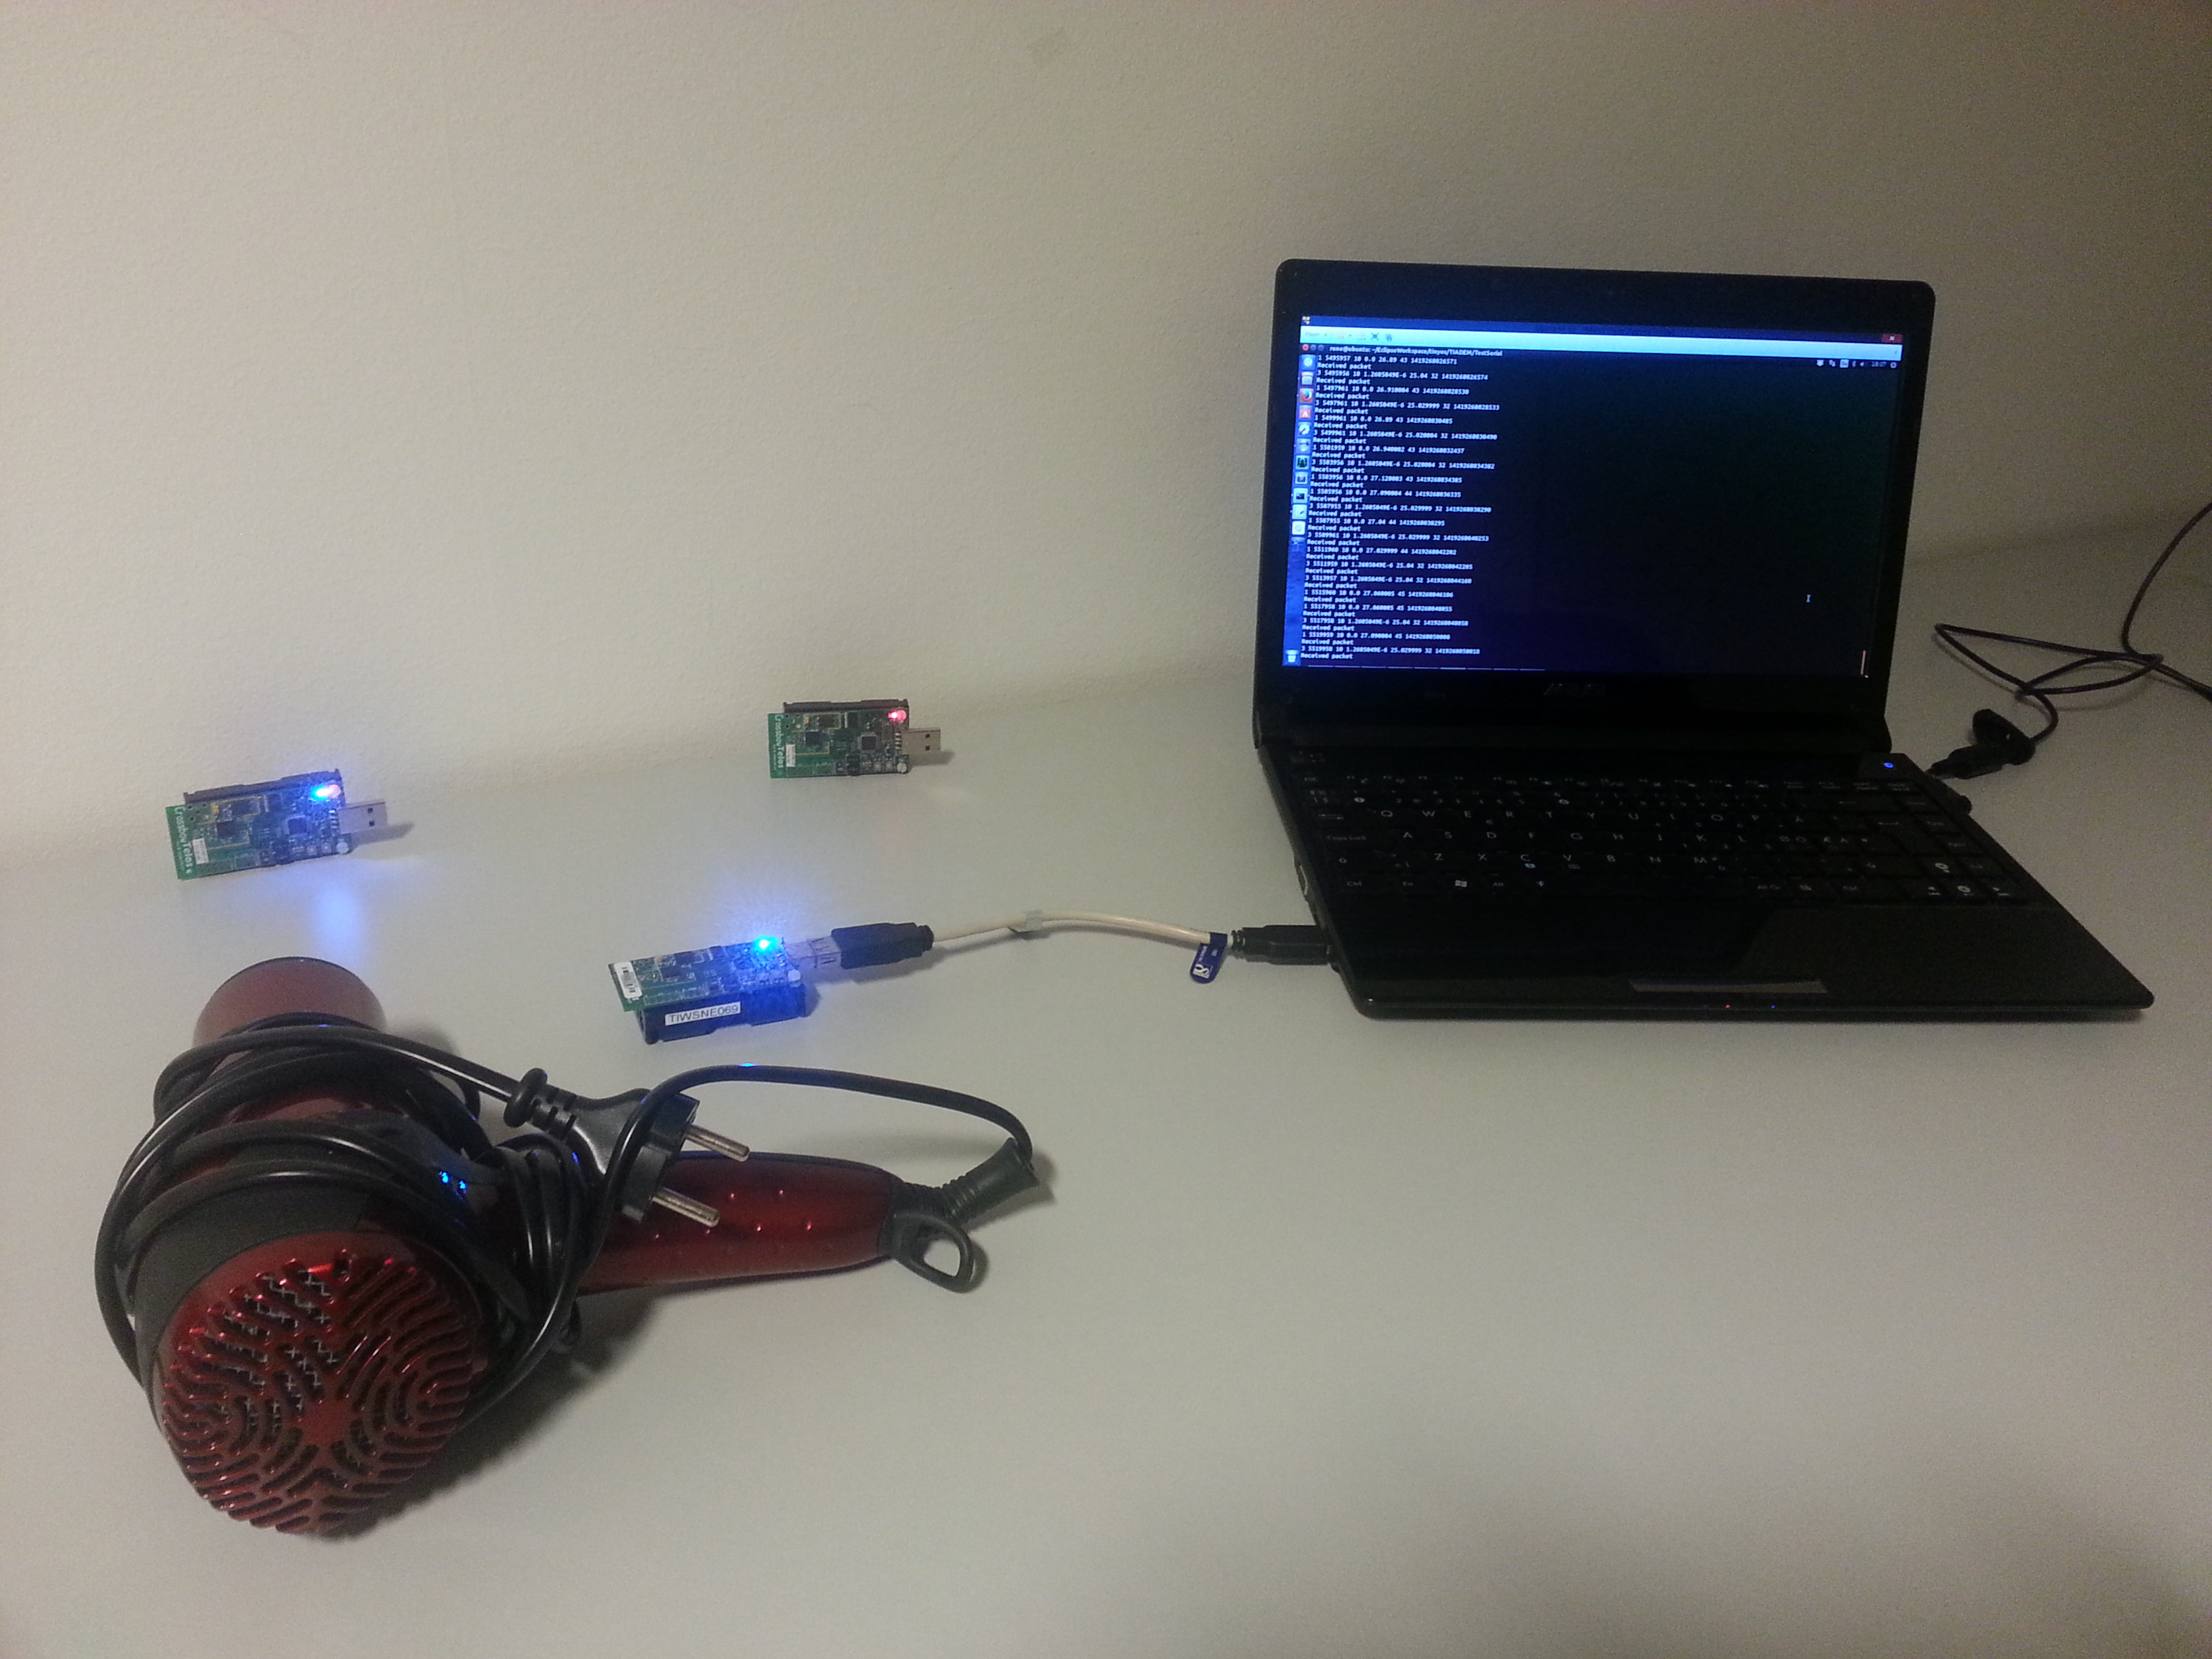
\includegraphics[width=\linewidth]{TestSetup.jpg}
			\caption{Test Setup}
			\label{fig:TestSetup}
		\end{figure}
	
	% subsection test_setup (end)

	\subsection{Test Results} % (fold)
	\label{sub:test_results}

		\subsubsection{Stable Environment} % (fold)
		\label{sub:stable_environment}
			
			\begin{figure}[H]
				\centering
				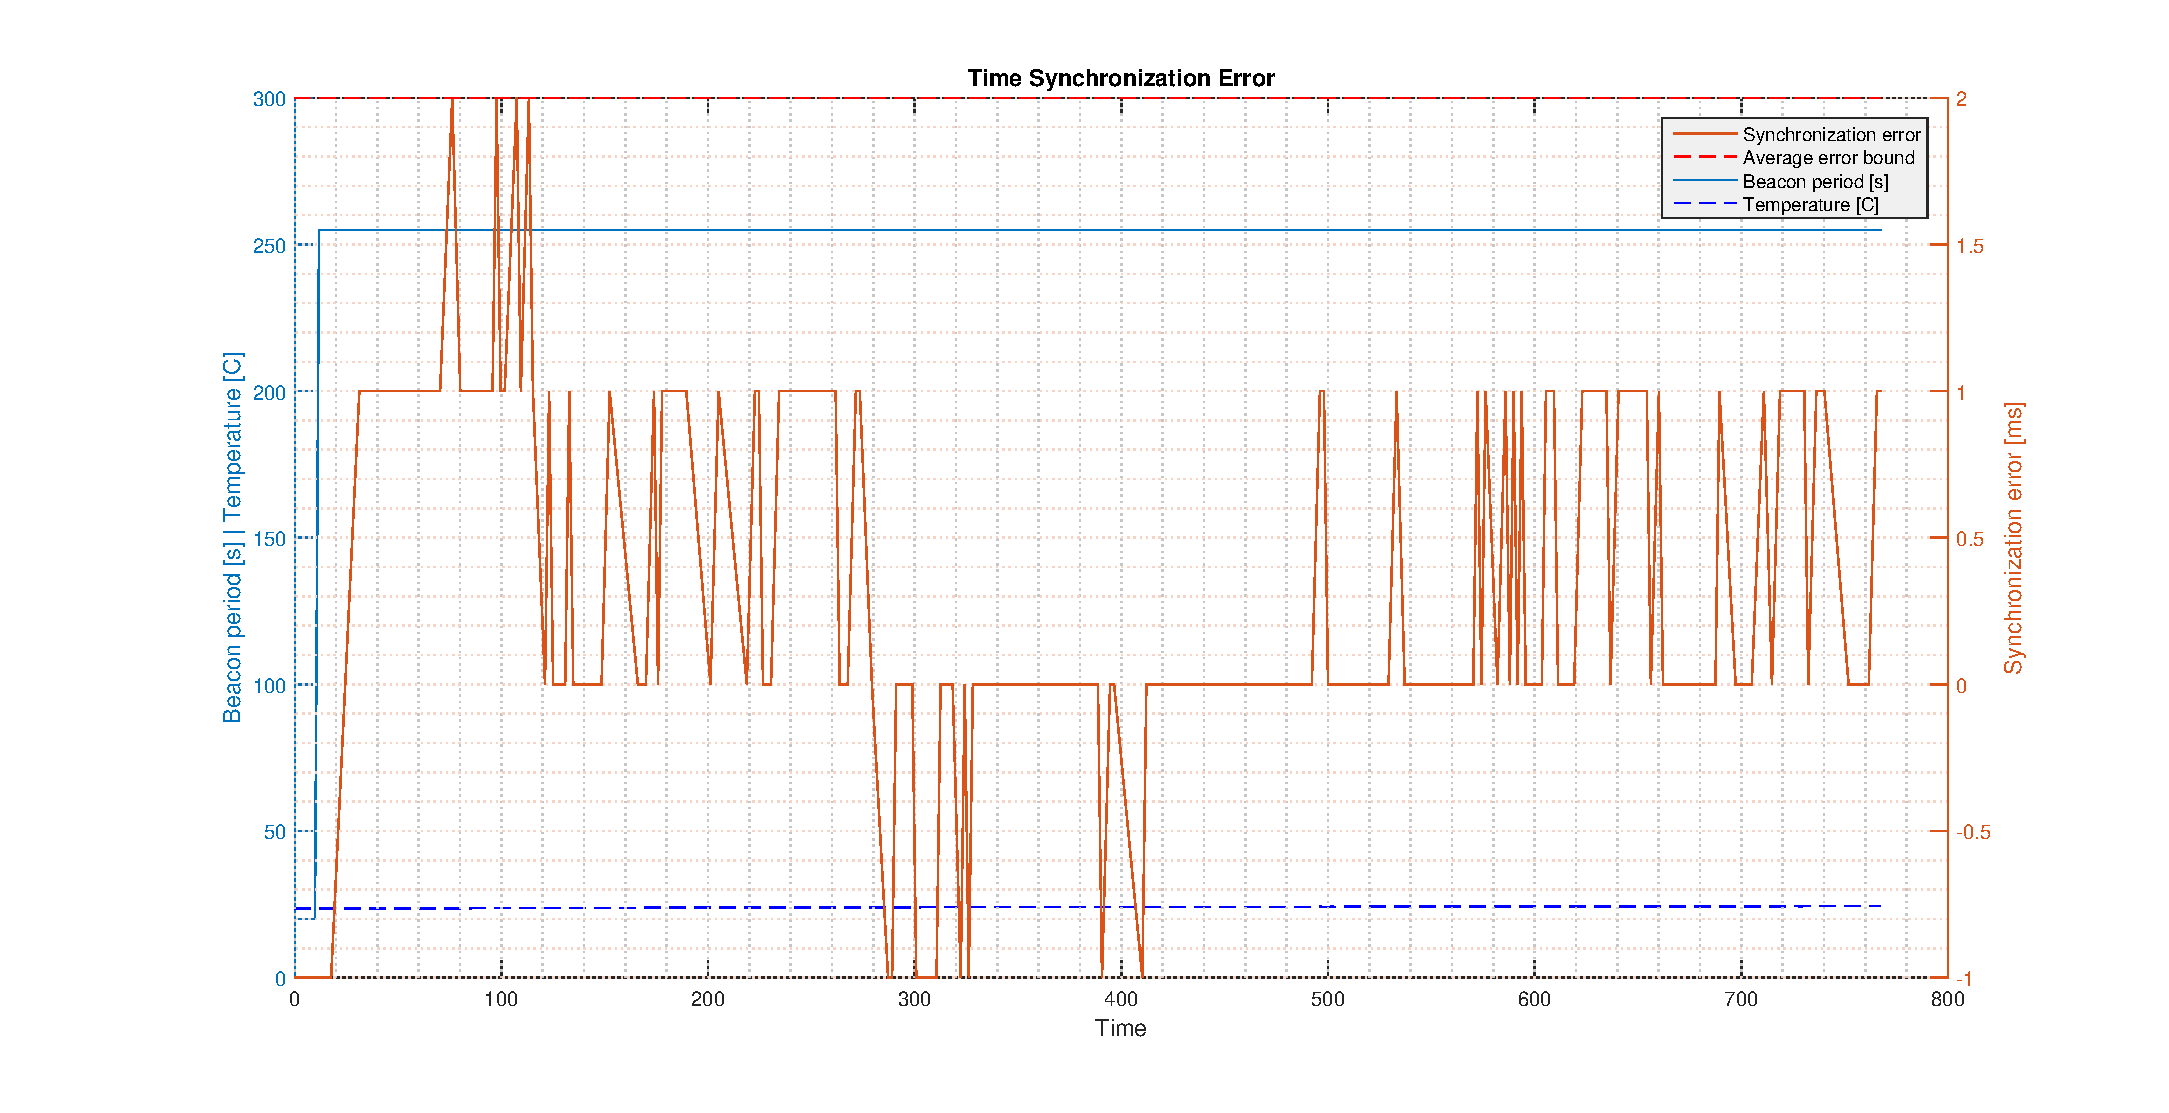
\includegraphics[width=\linewidth]{StableSynchronization.eps}
				\caption{Time Synchronization Error}
				\label{fig:Synchronization}
			\end{figure}

		% subsubsection stable_environment (end)

		\subsubsection{Unstable Environment} % (fold)
		\label{sub:unstable_environment}
			
			\begin{figure}[H]
				\centering
				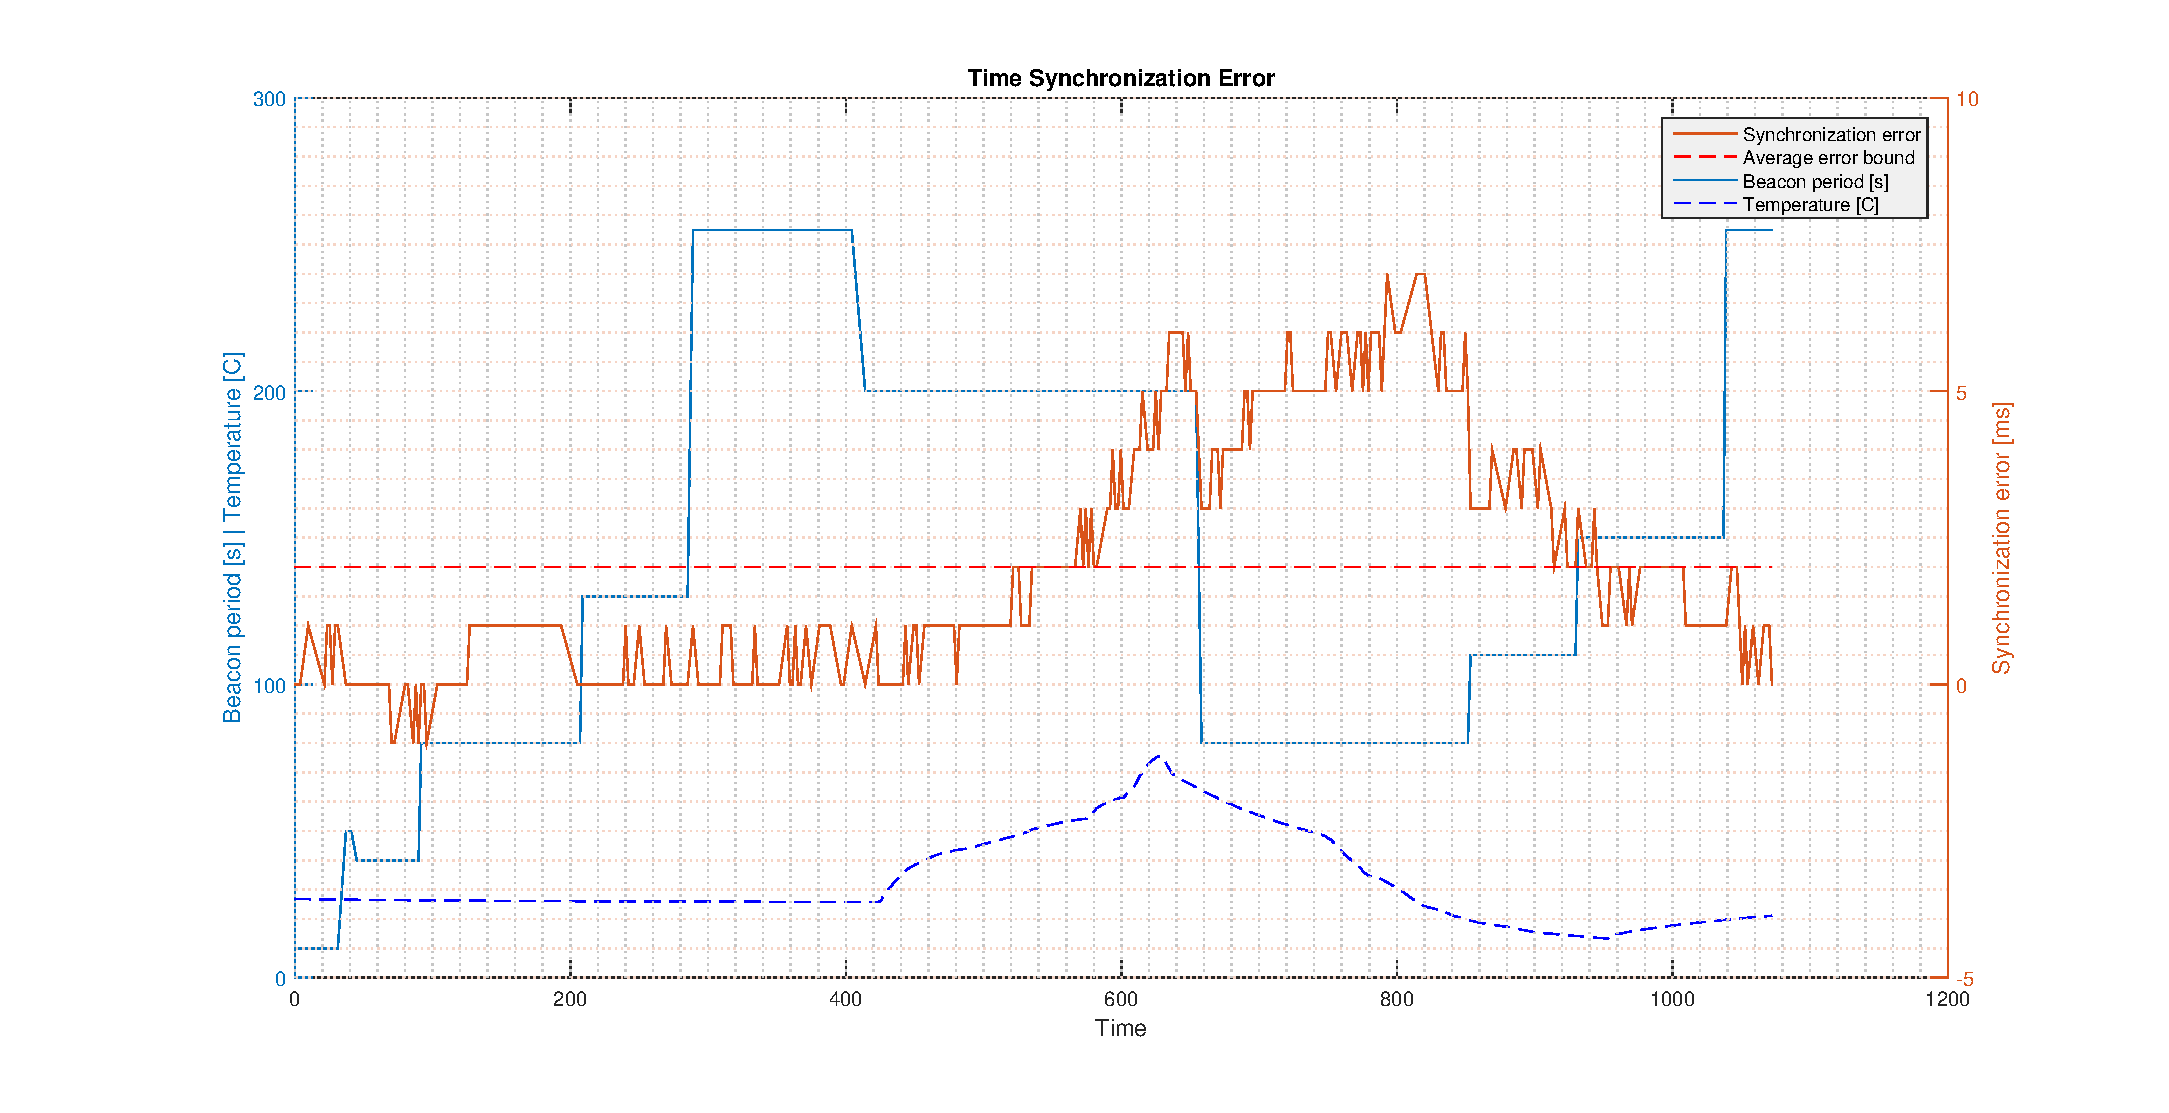
\includegraphics[width=\linewidth]{Synchronization.eps}
				\caption{Time Synchronization Error}
				\label{fig:Synchronization}
			\end{figure}

		% subsubsection unstable_environment (end)
	
	% subsection test_results (end)

% section contribution (end)

\end{document}
